Hyperledger incubates and promotes a range of business blockchain technologies. These technologies include:  \begin{itemize}
\item Distributed ledger frameworks 
\item Smart contract engines 
\item Client libraries 
\item Graphical interfaces 
\item Utility libraries
\item Sample applications 
\end{itemize}

The Hyperledger umbrella strategy encourages the re-use of common building blocks, enables rapid innovation of components, and promotes interoperability between projects.  

Table X sums up all the current projects, in chronological order from the date they were accepted by  Hyperledger. The rest of this section sums up each project briefly, and shows where to find more information. 

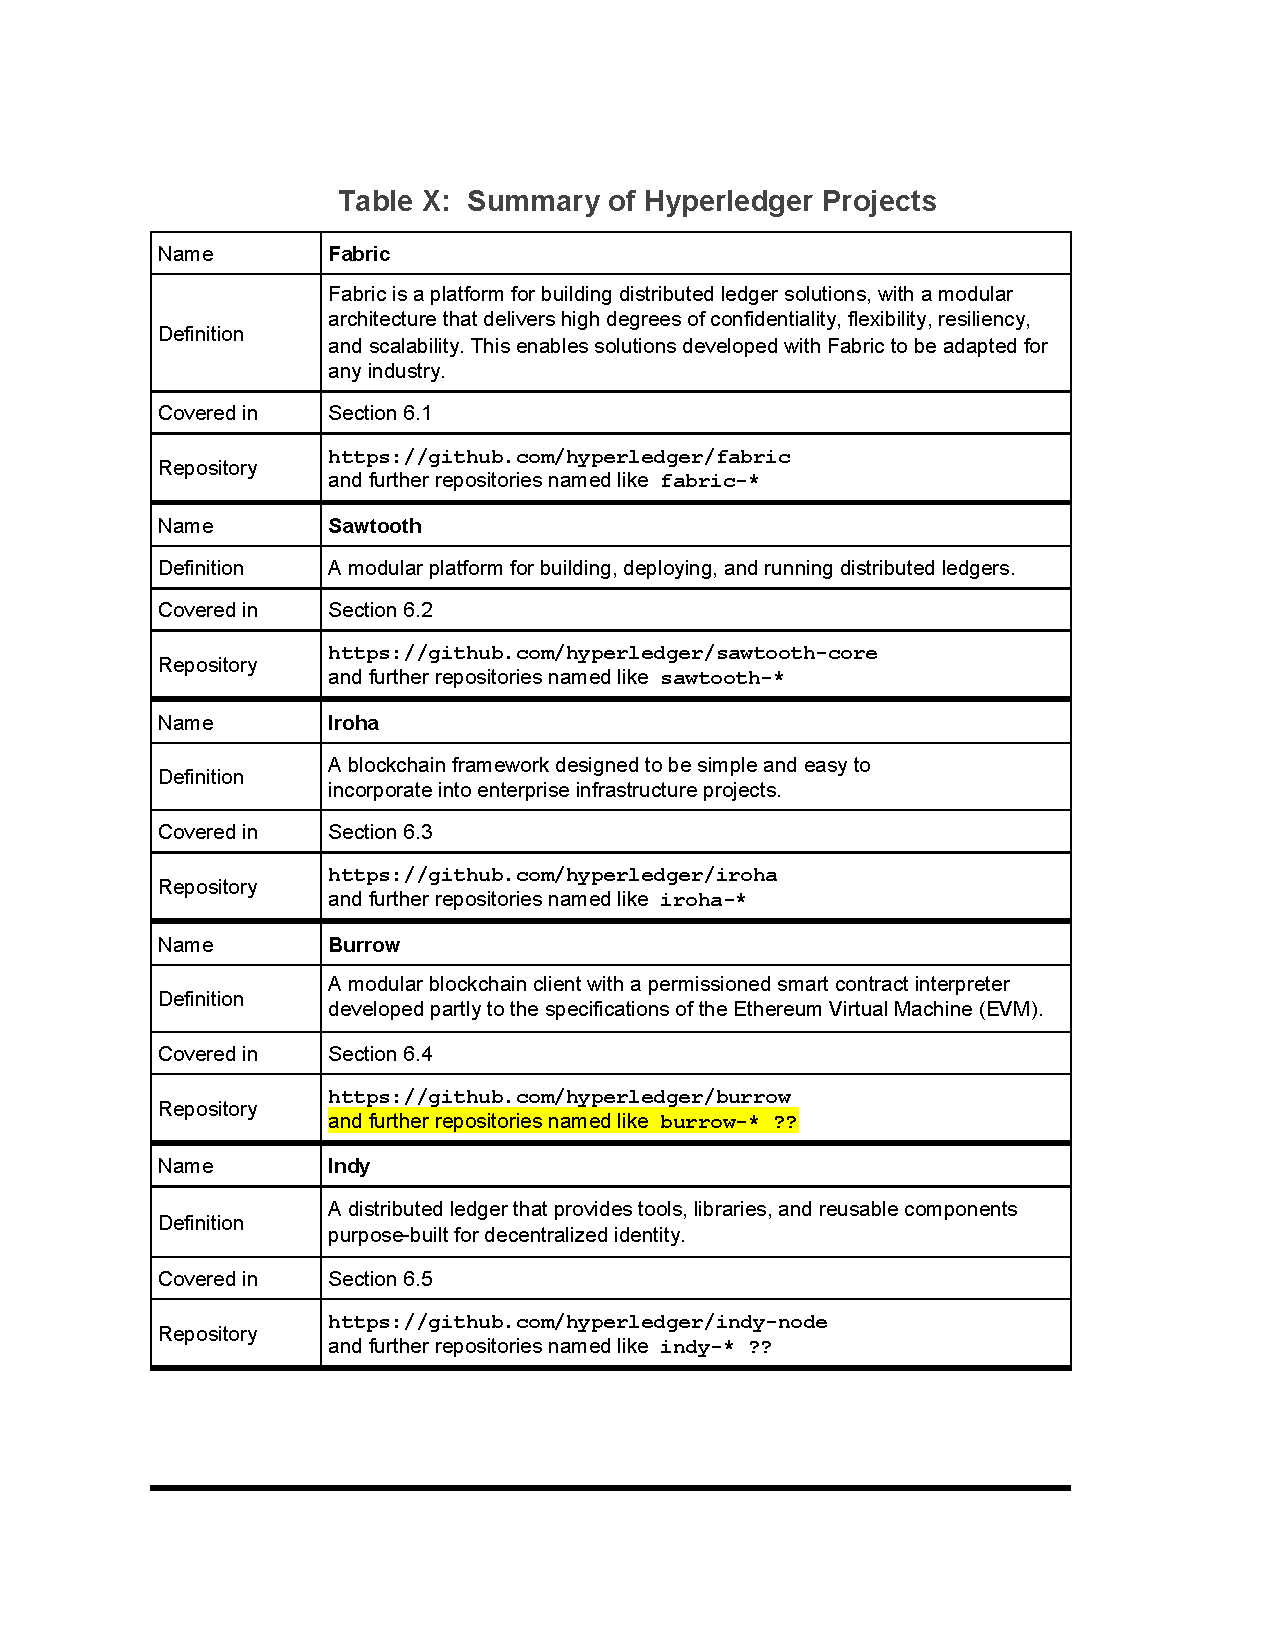
\includepdf{CurrentProjects/summary_of_hyperledger_projects_page1.pdf}

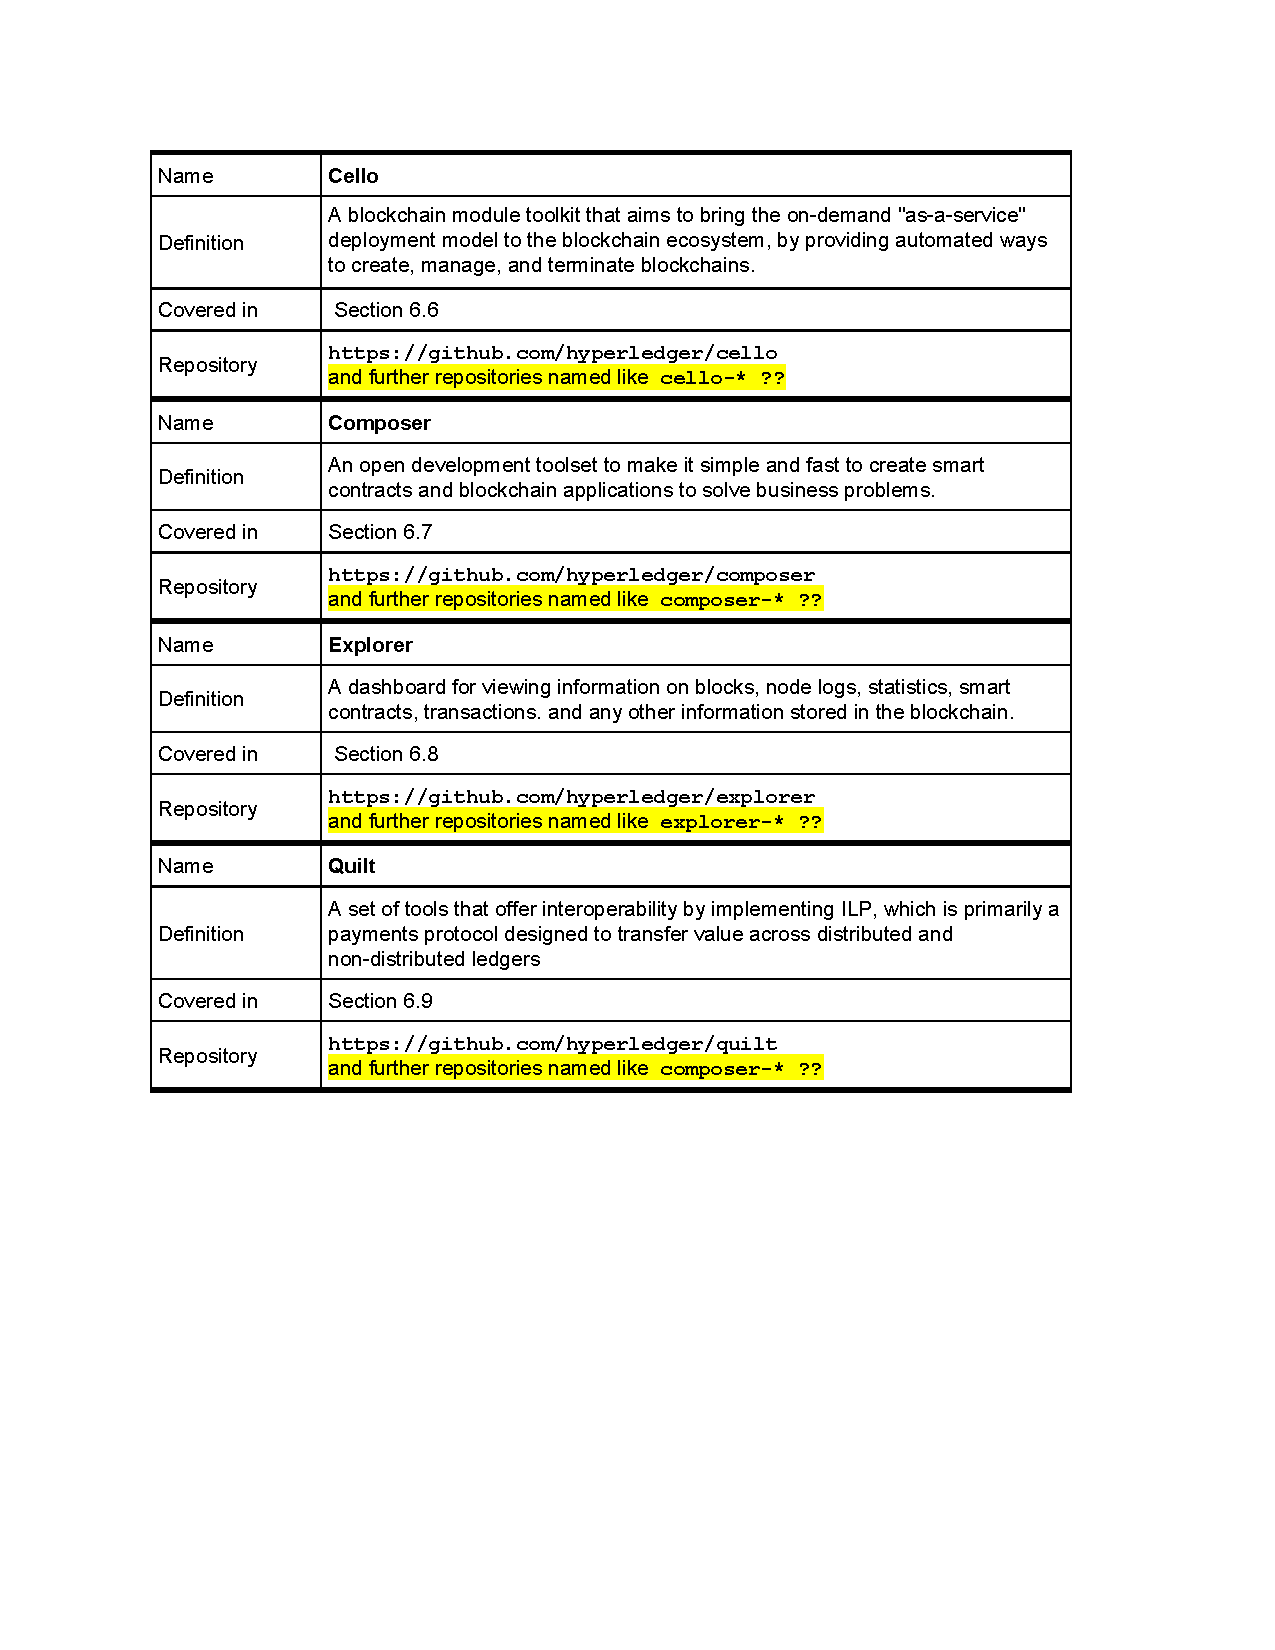
\includepdf{CurrentProjects/summary_of_hyperledger_projects_page2.pdf}

\subsection{Fabric}
Hyperledger Fabric (\url{https://github.com/hyperledger/fabric} and further repositories named like \url{fabric-*}) is a platform for distributed ledger solutions, underpinned by a modular architecture delivering high degrees of confidentiality, resiliency, flexibility and scalability. It is designed to support pluggable implementations of different components, and to accommodate the complexity and intricacies that exist across the economic ecosystem.

Starting from the premise that there are no ``one-size-fits-all'' solutions, Fabric is an extensible blockchain platform for running distributed applications.  It supports modular consensus protocols, which allows the system to be tailored to particular use cases and trust models. Fabric runs distributed applications written in general-purpose programming languages, without systemic dependency on a native cryptocurrency.  This stands in sharp contrast to most other blockchain platforms for running smart contracts that require code to be written in domain-specific languages or rely on a cryptocurrency.  Furthermore, it uses a portable notion of membership for realizing the permissioned model, which may be integrated with industry-standard identity management.  To support such flexibility, Fabric takes a novel architectural approach and revamps the way blockchains cope with non-determinism, resource exhaustion, and performance attacks.

%Where Hyperledger Fabric breaks from some other blockchain systems is that it is private and permissioned. Rather than allowing anyone to be part of the network by either participating in the Proof-of-Work consensus or receiving transferrable forms of data such as tokens over the blockchain, the members of a Hyperledger Fabric network enroll through a membership services provider.

Fabric also offers the ability to create channels, allowing a group of participants to create a separate ledger of transactions. This is an especially important option for networks where some participants might be competitors and not want every transaction they make, such as a special price they’re offering to some participants and not others, known to every participant in the network. If a group of participants form a channel, then only those participants, and no others, have copies of the ledger for that channel.



\subsection{Sawtooth}
Hyperledger Sawtooth (\url{https://github.com/hyperledger/sawtooth-core} and further repositories named like \url{sawtooth-*}) is a modular platform for building, deploying, and running distributed ledgers. The Sawtooth design philosophy targets keeping distributed ledgers distributed and making smart contracts safe - particularly for enterprise use.

In fitting with this enterprise focus, Sawtooth is also highly modular. This enables enterprises and consortia to make policy decisions that they are best equipped to make.

Originally, Sawtooth was designed to explore scalability, security, and privacy questions prompted by the original distributed ledgers. That mandated a certain modularity that was lacking at the time. Starting from scratch allowed us to employ lessons from those pioneering systems and branch into usages that the original currency ledgers weren’t intended to address. PoET, the new consensus hits scalability, while Transaction Families, our contract logic, narrow the attack surface for contracts while simultaneously broadening the functionality. We also have a keen interest in trusted execution environments and what role that can play in private transactions.

In branching into new business cases, we felt it was important that the system preserve certain tenants of a distributed ledger. That is, in an enterprise deployment, the concept of a distributed ledger shouldn’t collapse into a replicated database. Enterprise participants need autonomy and they have the right to run their own nodes. The set of participants will also be dynamic and the system – particularly consensus – must accommodate that volatility. It is not clear, for example, whether an O(n2) protocol with fixed membership like PBFT can support the scale or volatility of a distributed ledger at production levels. Further it seems inadvisable to sidestep the challenges of providing Byzantine Fault Tolerance and operate on only a Crash Fault Tolerant consensus. Finally, we observed that, “public” and “private” define a spectrum of authorization policies – not a binary option for a distributed ledger.


\subsection{Iroha}
Hyperledger Iroha (\url{https://github.com/hyperledger/iroha}) joined Hyperledger Fabric and Hyperledger Sawtooth to become the third distributed ledger platform under the Hyperledger umbrella in October, 2016. It was originally developed by Soramitsu in Japan and was proposed to Hyperledger by Soramitsu, Hitachi, NTT Data, and Colu.

Hyperledger Iroha is designed to be simple and easy to incorporate into infrastructural projects requires distributed ledger technology. Hyperledger Iroha features a simple construction; modern, domain-driven C++ design, emphasis on mobile application development and a new, chain-based Byzantine Fault Tolerant consensus algorithm, called Sumeragi. 

Iroha takes a very different design philosophy from Hyperledger Fabric and Hyperledger Sawtooth, in that it focuses on providing features that are helpful for creating applications for end-users. 


\subsection{Burrow}
Hyperledger Burrow is a permissionable smart contract machine; it became the fourth distributed ledger platform under the Hyperledger umbrella in April, 2017. It was originally developed and proposed to Hyperledger by Monax. 

Burrow provides a modular blockchain client with a permissioned smart contract interpreter built to the specification of the Ethereum Virtual Machine (EVM). Burrow provides a strongly deterministic, smart contract focused, blockchain design to Hyperledger's overall effort. Users of Burrow are able to benefit from having an access control layer through the use of smart contracts and our “secure natives” based permission layer. 
 
The major components of Burrow are as follows:
 
Consensus engine which is responsible for maintaining the networking stack between nodes and ordering transactions to be utilized by the application engine.
Application Blockchain Interface (“ABCI”) provides the interface specification for the consensus engine and application engine to connect.
Smart contract application engine provides application builders with a strongly deterministic smart contract engine for operating complex industrial processes.
Gateway provides programmatic interfaces for systems integrations and user interfaces


\subsection{Indy}
Hyperledger Indy uses distributed ledger technology to make identity independent of organizational silos; friends, competitors, and even antagonists can all rely on a shared source of truth that answers fundamental questions such as, “Who am I dealing with?” and “How can I verify data about the other party in this interaction?” Solid answers to these questions enable the sort of trusted interactions demanded everywhere.

Because Indy stores identity artifacts (public keys, proofs of existence, cryptographic accumulators that enable revocation) on a ledger with distributed ownership, identities can be self-sovereign--nobody external to the identity owner can manipulate them or take them away. Identity in Indy is also privacy-preserving by default, meaning that an identity owner can operate without creating correlation risk or breadcrumbs.

A core technology for Indy is verifiable claims. These attestations of an identity’s attributes resemble credentials familiar to all of us: passports, driver’s licenses, birth certificates, and so forth. But they can be combined and transformed in powerful ways, using zero-knowledge proofs to enable selective disclosure of just those pieces of data that a particular context demands.

This combination of self-sovereignty, privacy, and verifiable claims is synergistic. Bulk troves of sensitive data vanish or become useless. The economics of hacking transform. The competing demands of privacy-preserving and strongly identifying regulations are satisfied. Individuals and organizations are free to seek mutual benefit from rich interaction; the identity ecosystem gains the innovation and dynamism of a free market. 

Despite the advanced crypto under the hood, Indy’s API is simple and straightforward. It consists of about 50 C-callable functions, with idomatic wrappers for many mainstream programming languages, 



\subsection{Cello}
Hyperledger Cello is an open framework to help people adopt blockchain technologies efficiently and easily, by providing automatic ways in blockchain provision and operational management. 

It brings the on-demand "as-a-service" deployment model to the blockchain ecosystem to reduce the effort required for maintaining the lifecycle of the Hyperledger blockchain frameworks. It provides a multi-tenant chain service efficiently and automatically on top of various infrastructures, including baremetal, virtual machine, Cloud platforms like AWS, and container platforms like Docker Swarm and Kubernetes, overall helping provide "Blockchain as a Service" efficiently. It also helps with maintainance through a dashboard where users can watch the statistics/status of the blockchain system (e.g., system utilization, blockchain events, chaincode performance), and manage the blockchains (e.g., create, config and delete) and chaincode (e.g., deploy and upload private chaincode) in real-time.

Hyperledger Cello currently supports Hyperledger Fabric 1.0 as the main blockchain implementation, while it has plans to support more blockchain types like sawtooth. The architecture follows the micro-service style, with pluggable implementations for most components. The main programing languages are Python and JavaScript.


\subsection{Composer}
TODO.

\subsection{Explorer}
Hyperledger Explorer (\url{https://github.com/hyperledger/blockchain-explorer}) provides a dashboard for viewing information about transactions, blocks, node logs, statistics,  and smart contracts available on the network. Users will be able to query for specific blocks or transactions and view the complete details. Blockchain explorer can also be integrated with any authentication/authorization platforms (commercial/open source) and will provided appropriate functionality based on the privileges available to the user. 
Goals of the project are listed below.
To implement a generic Blockchain explorer web application which is easy to install and can be used with different Blockchain platforms.
Use latest tools and technologies that make the explorer easy to implement, maintain and extend.
Easily installable package available through standard package managers for most popular platforms.

%Please refer to the project proposal document on the wiki (\url{https://wiki.hyperledger.org/projects/explorer}) page to understand more about the project.


\subsection{Quilt: coming soon}
\textbf{Hyperledger Quilt} offers interoperability between ledger systems by implementing the Interledger Protocol (ILP), a payments protocol designed to transfer value across both distributed and non-distributed ledgers. 

At the publication date of this document, Hyperledger Quilt was coming soon. 

\subsubsection{About the ILP}
Payment networks today are siloed and disconnected. 
Because of this, while payments are relatively easy within one country, or if both the sender and recipient have accounts on the same network or ledger, sending from one ledger to another is often impossible. 
Where connections do exist, they are manual, slow, or expensive.

The Interledger Protocol provides for routing payments across different digital asset ledgers, while isolating senders and receivers from the risk of intermediary failures. Secure multi-hop payments and automatic routing enable a global network of networks for different types of value that can connect any sender with any receiver.

\subsubsection{For more information}
To find out more about ILP, visit \url{https://interledger.org/rfcs/0003-interledger-protocol/}.

To see more about Hyperledger Quilt, visit the Projects webpage at \url{https://www.hyperledger.org/projects#}.

%\Or see \url{https://github.com/hyperledger/quilt} and further repositories named like \url{quilt-*}. 








\end{document}